
                                                                               \documentclass[tikz]{standalone}
\usepackage{lmodern}
\usepackage[algoruled,vlined,linesnumbered,titlenotnumbered,noend]{algorithm2e}
\usepackage{color,amsmath,bm,bbm,stmaryrd,amssymb,pifont,bbding}
\usetikzlibrary{backgrounds}
\usetikzlibrary{calc} 

\usetikzlibrary{shapes}
\usetikzlibrary{shadows}
\usetikzlibrary{decorations.pathmorphing}
\usetikzlibrary{decorations.text}
\usetikzlibrary{decorations}
\usetikzlibrary{arrows,bending}
\usetikzlibrary{shapes.arrows}
\tikzset{nobg/.style={show background rectangle,background rectangle/.style={opacity=0}}}


\input ../../styles
\input ../../globalcomm
\input ../../localcomm
\usetikzlibrary{arrows, shapes.gates.logic.US, calc}

  \tikzstyle{bddnode}=[draw,rectangle,rounded corners=2mm]
  \tikzstyle{aops}=[pos=0.9,below,yshift=0mm,xshift=-2mm]
\begin{document}



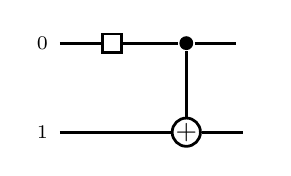
\begin{tikzpicture}[line width=1pt]
\node[name=x1]{$\ketof{\xvar_0}$};
\node[name=x2,anchor=north] at 
($(x1.south)+(0pt,-20pt)$){$\ketof{\xvar_1}$};

\node[name=H,anchor=west,draw] at 
($(x1.east)+(15pt,0pt)$){$\hgate$};
\node[name=cnot1,anchor=west,circle,fill,inner sep=0pt,minimum size=5pt] at 
($(H.east)+(20pt,0pt)$){};
\node[name=cnot2,circle,draw,inner sep=0pt] at 
(cnot1|-x2){$+$};

\node[anchor=west,name=end1] at ($(cnot1.east)+(15pt,0pt)$){};
\node[anchor=west,name=end2] at ($(cnot2.east)+(15pt,0pt)$){};

\draw (x1) -- (H);
\draw (H) -- (cnot1);
\draw (x2) -- (cnot2);
\draw (cnot1) -- (cnot2);
\draw (cnot1) -- (end1);
\draw (cnot2) -- (end2);
\end{tikzpicture}

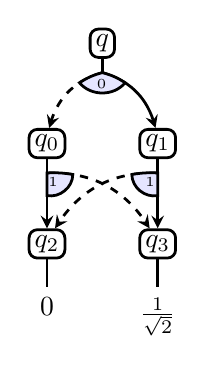
\begin{tikzpicture}[line width=1pt]
%%%%%%%%%%%%%%% p: root %%%%%%%%%%%%%%%%%%%
\node[draw,rectangle,inner sep=2pt,rounded corners=3pt] (q) {$q$};
\coordinate (qB) at ($(q.south)+(0pt,-5pt)$);
\draw (q) -- (qB);


%%%%%%%%%%%%%%% Level 1 %%%%%%%%%%%%%%%%%%%

\node[draw,rectangle,inner sep=2pt,rounded corners=3pt,anchor=north,name=q0] 
at ($(qB)+(-20pt,-20pt)$){$q_0$};
\node[draw,rectangle,inner sep=2pt,rounded corners=3pt,anchor=north,name=q1] 
at ($(qB)+(20pt,-20pt)$){$q_1$};

\coordinate (q0B) at ($(q0.south)+(0pt,-5pt)$);
\draw (q0) -- (q0B);
\coordinate (q1B) at ($(q1.south)+(0pt,-5pt)$);
\draw (q1) -- (q1B);



\draw[bend right=30,->,>=stealth,dashed](qB) to coordinate[pos=0.3] (qBlm)(q0);
\draw[bend left=30,->,>=stealth](qB) to coordinate[pos=0.3] (qBrm)(q1);
\draw[fill=blue!10] (qB) to [bend right=9]  (qBlm) to [bend right=50]  (qBrm) to [bend right=9] cycle;


%%%%%%%%%%%%%%% Level 2 %%%%%%%%%%%%%%%%%%%

\node[draw,rectangle,inner sep=2pt,rounded corners=3pt,anchor=north,name=q2] 
at ($(q0B)+(0pt,-20pt)$){$q_2$};
\node[draw,rectangle,inner sep=2pt,rounded corners=3pt,anchor=north,name=q3] 
at ($(q1B)+(0pt,-20pt)$){$q_3$};

\node[anchor=north,name=q2B] at ($(q2.south)+(0pt,-10pt)$) {$0$};;
\draw (q2) -- (q2B);
\node[anchor=north,name=q3B] at ($(q3.south)+(0pt,-10pt)$) {$\frac1{\sqrt2}$};;
\draw (q3) -- (q3B);


\draw[bend left=0,->,>=stealth](q0B) to coordinate[pos=0.4] (q0Blm)(q2);
\draw[bend left=30,->,>=stealth,dashed](q0B) to coordinate[pos=0.2] (q0Brm)(q3);
\draw[fill=blue!10] (q0B) to [bend right=0]  (q0Blm) to [bend right=50]  (q0Brm) to [bend right=6] cycle;


\draw[bend left=0,->,>=stealth](q1B) to coordinate[pos=0.4] (q1Blm)(q3);
\draw[bend right=30,->,>=stealth,dashed](q1B) to coordinate[pos=0.2] (q1Brm)(q2);
\draw[fill=blue!10] (q1B) to [bend left=0]  (q1Blm) to [bend left=50]  (q1Brm) to [bend left=6] cycle;


\node[anchor=north,inner sep=2pt,font=\tiny]at(qB.south){$\xvar_0$};
\node[anchor=north west,inner sep=0pt,font=\tiny]at($(q0B.south)+(0pt,-1pt)$){$\xvar_1$};
\node[anchor=north east,inner sep=0pt,font=\tiny]at($(q1B.south)+(0pt,-1pt)$){$\xvar_1$};

\end{tikzpicture}


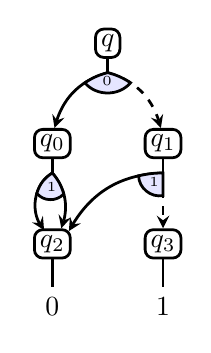
\begin{tikzpicture}[line width=1pt]
%%%%%%%%%%%%%%% p: root %%%%%%%%%%%%%%%%%%%
\node[draw,rectangle,inner sep=2pt,rounded corners=3pt] (q) {$q$};

\coordinate (qB) at ($(q.south)+(0pt,-5pt)$);
\draw (q) -- (qB);



%%%%%%%%%%%%%%% Level 1 %%%%%%%%%%%%%%%%%%%

\node[draw,rectangle,inner sep=2pt,rounded corners=3pt,anchor=north,name=q0] 
at ($(qB)+(-20pt,-20pt)$){$q_0$};
\node[draw,rectangle,inner sep=2pt,rounded corners=3pt,anchor=north,name=q1] 
at ($(qB)+(20pt,-20pt)$){$q_1$};

\coordinate (q0B) at ($(q0.south)+(0pt,-5pt)$);
\draw (q0) -- (q0B);
\coordinate (q1B) at ($(q1.south)+(0pt,-5pt)$);
\draw (q1) -- (q1B);



\draw[bend right=30,->,>=stealth](qB) to coordinate[pos=0.3] (qBlm)(q0);
\draw[bend left=30,->,>=stealth,dashed](qB) to coordinate[pos=0.3] (qBrm)(q1);
\draw[fill=blue!10] (qB) to [bend right=9]  (qBlm) to [bend right=50]  (qBrm) to [bend right=9] cycle;

\node[anchor=north,inner sep=1pt,font=\tiny]at(qB.south){$\xvar_0$};

%%%%%%%%%%%%%%% Level 2 %%%%%%%%%%%%%%%%%%%

\node[draw,rectangle,inner sep=2pt,rounded corners=3pt,anchor=north,name=q2] 
at ($(q0B)+(0pt,-20pt)$){$q_2$};
\node[draw,rectangle,inner sep=2pt,rounded corners=3pt,anchor=north,name=q3] 
at ($(q1B)+(0pt,-20pt)$){$q_3$};

\node[anchor=north,name=q2B] at ($(q2.south)+(0pt,-10pt)$) {$0$};;
\draw (q2) -- (q2B);
\node[anchor=north,name=q3B] at ($(q3.south)+(0pt,-10pt)$) {$1$};;
\draw (q3) -- (q3B);


\draw[bend left=30,->,>=stealth](q0B) to coordinate[pos=0.4] (q0Blm)(q2);
\draw[bend right=50,->,>=stealth](q0B) to coordinate[pos=0.4] (q0Brm)($(q2)+(-3pt,5pt)$);
\draw[fill=blue!10] (q0B) to [bend left=12]  (q0Blm) to [bend left=50]  (q0Brm) to [bend left=20] cycle;

\node[anchor=north,inner sep=3pt,font=\tiny]at(q0B.south){$\xvar_1$};

\draw[bend left=0,->,>=stealth,dashed](q1B) to coordinate[pos=0.4] (q1Blm)(q3);
\draw[bend right=30,->,>=stealth](q1B) to coordinate[pos=0.2] (q1Brm)($(q2.north east)+(-1pt,-1pt)$);
\draw[fill=blue!10] (q1B) to [bend left=0]  (q1Blm) to [bend left=50]  (q1Brm) to [bend left=6] cycle;

\node[anchor=north,inner sep=3pt,font=\tiny]at
($(q1B.south)+(-3pt,2pt)$){$\xvar_1$};


\end{tikzpicture}

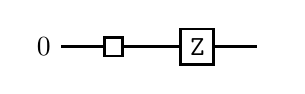
\begin{tikzpicture}[line width=1pt]
\node[name=in0]{$\ketof{0}$};


\node[name=H,anchor=west,draw] at 
($(in0.east)+(15pt,0pt)$){$\hgate$};
\node[name=Z,anchor=west,draw] at 
($(H.east)+(20pt,0pt)$){${\mathtt Z}$};


\node[anchor=west,name=end] at ($(Z.east)+(15pt,0pt)$){};


\draw (in0) -- (H);
\draw (H) -- (Z);
\draw (Z) -- (end);
\end{tikzpicture}



\end{document}

